\chapter{Evaluation}

\section{Document management}

In this section, we take table~\ref{tab:background-comparison} as a starting
point and check what features are implemented and what are not.

The testing environment was built from a client machine, a SharePoint server
and an Alfresco server, as can be seen on figure~\ref{fig:test-arch}.

\begin{figure}[H]
\centering
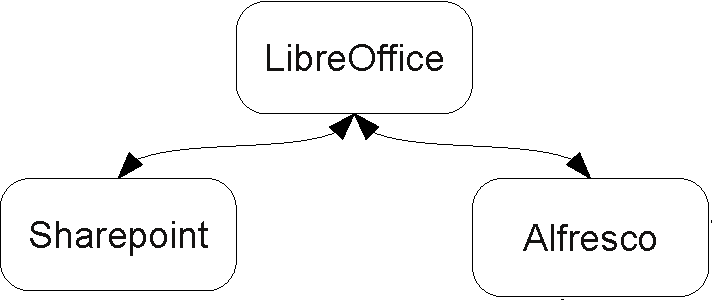
\includegraphics[width=300px,keepaspectratio]{test-arch.pdf}
\caption{Architecture of the test system}
\label{fig:test-arch}
\end{figure}

The client machine had the following details:
\begin{itemize}
\item Frugalware Linux 1.5 (English and Hungarian locale)
\item LibreOffice 3.4, LibreOffice 3.3, OpenOffice.org 3.3 and OpenOffice.org 3.2.1
\end{itemize}

Properties of the SharePoint machine:

\begin{itemize}
\item Microsoft Windows Windows Server 2003 R2 Enterprise (English)
\item Microsoft SharePoint 2007 Enterprise
\end{itemize}

Finally the Alfresco machine:

\begin{itemize}
\item Fedora Linux 16
\item Alfresco 3.4.d Community Edition
\end{itemize}

Regarding functionality, all items from the feature table are implemented in
the extension. The following areas are missing from the table, and not
supported at the moment:

\begin{itemize}
\item User management, including roles and permissions inside workspaces.
\item Task management in workspaces.
\item Link management in workspaces.
\end{itemize}

The following items are not in the feature table, but are available:

\begin{itemize}
\item Creating and deleting workspaces is supported by Microsoft Office, but nested
folder structures can only be read. It turned out that the protocol allows
creation, so the extension supports this.
\item Namespaces of settings and classes are renamed, so parallel installation
of our extension and OPAL is possible.
\end{itemize}

The extension is written in Java and BASIC, so it is meant to be portable.
LibreOffice is available on Windows and OSX as well -- so the extension should
work there, but we only had time to test it on Windows.

Regarding localization, all user-visible strings are externalized to Java
property files. During development we paid attention to English strings, then at
the end as a demonstration we created the Hungarian translation as well. Adding
new translations is easy.

Finally, the extension inherited some of its limitation from the original OPAL
codebase:

\begin{itemize}
\item The GUI is not started in a separate thread in all cases, resulting the
lack of the update of the user interface background in many cases.
\item Classes we did not touch still have French comments inside.
\end{itemize}

\section{Workflows}

\subsection*{Test architecture}

The evaluation of workflow support is based on the use-cases of the workflow
part of the \emph{Overview of the Approach} chapter.

\begin{figure}[H]
\centering
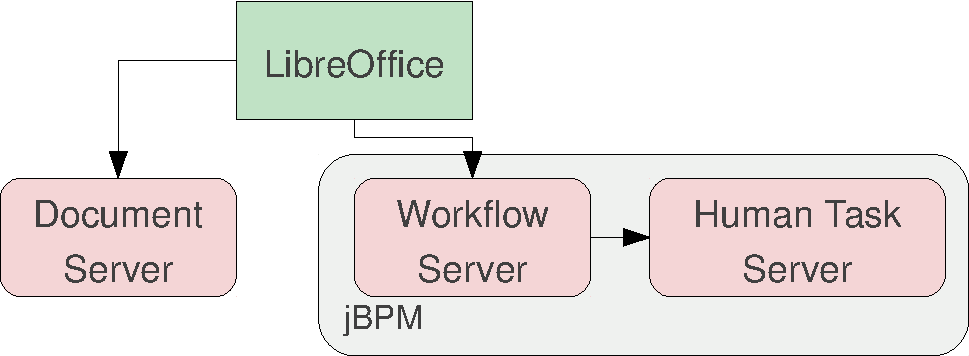
\includegraphics[width=300px,keepaspectratio]{test-arch-wf.pdf}
\caption{Architecture of the workflow-enabled test system}
\label{fig:test-arch-wf}
\end{figure}

The test architecture we designed to evaluate features can be seen on
figure~\ref{fig:test-arch-wf}. The test system has the following dependencies:

\begin{itemize}
\item The connection should be initiated from our LibreOffice extension when
both the document server and the workflow engine is ready.
\item The workflow server can be started before the Human Task server, but user
connections can only be served when both are ready.
\item Additionally, in case a custom storage backend is used for jBPM (for
example MySQL instead of the default H2 backend), then that should be ready
before any component of jBPM is started.
\end{itemize}

During our tests we used the same document servers and office suites than for
the document-server-only tests. jBPM was set up on the same physical machine
where the office suite ran.

The workflow-specific tests were executed using the following component versions:

\begin{itemize}
\item jBPM (jbpm-bpmn2 and jbpm-human-task) 5.1.x: latest version at the time
of writing (Nov 2011) with additional patches detailed earlier.
\item BPM Console 2.1 with the patches.
\item MySQL 5.5.14 without additional modifications.
\end{itemize}

The jBPM developers are looking forward to the modifications and are planning
to review them once the thesis is ready.

\subsection*{Used test methods}

Foo.
